\documentclass[12pt,a4paper]{article}

\usepackage[margin=1in]{geometry}
\usepackage{graphicx}
\usepackage{array}
\usepackage{booktabs}
\usepackage{longtable}
\usepackage{enumitem}
\usepackage{xcolor}
\usepackage{hyperref}
\usepackage{tikz}
\usetikzlibrary{arrows.meta, positioning, shapes.geometric, fit, calc}

\hypersetup{
    colorlinks=true,
    linkcolor=blue,
    urlcolor=blue,
    citecolor=blue
}

\setlist[itemize]{leftmargin=1.2cm}
\setlist[enumerate]{leftmargin=1.2cm}

\title{\textbf{Mixed Reality AI Workspace Organizer}\\
\large Software Engineering Project Report}
\author{
    Name: \underline{\hspace{5cm}}\\
    Roll No.: \underline{\hspace{4.7cm}}\\
    Course: Software Engineering\\
    Institution: \underline{\hspace{4.2cm}}
}
\date{\today}

\begin{document}

\maketitle
\newpage

\tableofcontents
\newpage

\section{Abstract}

This project is a mixed reality workspace organization assistant developed in Unity for Meta Quest. The system uses Meta XR passthrough and object detection to understand the physical workspace visible to the user. It converts detected objects into structured scene data and sends this context to a locally hosted Ollama large language model. The model returns practical arrangement instructions such as where to place a laptop, keyboard, bottle, book, or other detected objects. The response is displayed in a Unity UI panel and can also be spoken using a Meta Text-to-Speech block with an ElevenLabs provider.

From a software engineering perspective, the project demonstrates modular design, event-driven architecture, client-ready scalability, requirement documentation, data flow modeling, agile planning, and safe integration of third-party AI services. The goal is not only to detect objects, but to create a usable and extensible assistant that can help users clean and organize real environments through voice and visual feedback.

\section{Introduction}

Cluttered workspaces reduce productivity and make it difficult for users to focus. A mixed reality device can see the user's physical environment and provide real-time guidance without requiring the user to manually describe every object. This project uses that idea to build an interactive assistant that observes objects in the user's environment, understands the user's request, and generates grounded organization suggestions.

The application currently supports two main modes:

\begin{itemize}
    \item \textbf{Voice-guided mode:} Pressing the X button starts speech-to-text. The user speaks a custom prompt, for example, ``I want this desk ready for studying.'' The system combines the spoken prompt with the detected scene and sends it to Ollama.
    \item \textbf{Default scene mode:} Pressing the Y button skips speech input and uses a default cleanup prompt. The system analyzes the detected objects and suggests how to make the space cleaner and more organized.
\end{itemize}

The system is designed as a prototype that can evolve into a client-facing product for students, office workers, accessibility support, inventory organization, and smart workspace assistance.

\section{Problem Statement}

The problem addressed by this project is the lack of context-aware, real-time assistance for organizing a physical workspace. Traditional task management applications require manual input and cannot directly understand the user's surroundings. General voice assistants can respond to spoken commands but usually do not know which objects are physically present in the room.

This project solves the problem by combining object detection, speech input, local language model reasoning, and mixed reality output. The user can look at a cluttered space, speak a goal, and receive object-specific placement instructions such as placing a laptop to the left of the keyboard or moving a bottle away from electronics.

\section{Project Objectives}

\begin{enumerate}
    \item Detect physical objects in the user's field of view using Meta XR object detection.
    \item Convert object detections into structured scene JSON containing labels, confidence, screen positions, zones, and object sizes.
    \item Accept user prompts through speech-to-text using the Meta XR speech block.
    \item Send scene context and user intent to a local Ollama model using HTTP requests.
    \item Generate useful, object-specific organization recommendations.
    \item Display recommendations in a Unity UI text panel for debugging and accessibility.
    \item Speak recommendations using Meta Text-to-Speech and ElevenLabs voice configuration.
    \item Keep the architecture modular so future clients can add new models, UI surfaces, prompts, and ghost placement features.
\end{enumerate}

\section{Scope}

\subsection{In Scope}

\begin{itemize}
    \item Meta Quest mixed reality passthrough setup.
    \item Object detection using the Meta XR object detection block and Sentis model asset.
    \item Local Ollama integration using the \texttt{llama3.2} model.
    \item Speech-to-text input through the Meta speech block.
    \item Text-to-speech output through the Meta TTS block and ElevenLabs provider.
    \item Unity UI text output for generated recommendations.
    \item Controller bindings for X and Y buttons.
    \item Software engineering documentation including SRS, DFD, architecture, testing, and agile plan.
\end{itemize}

\subsection{Out of Scope}

\begin{itemize}
    \item Fully automatic physical movement of real objects.
    \item Guaranteed detection of every object in the room.
    \item Cloud-hosted production backend.
    \item Enterprise user authentication and account management.
    \item Final polished commercial UI design.
\end{itemize}

\section{Existing System}

Current object detection or assistant systems generally operate as separate tools. Object detection systems can label objects, but they do not explain how to organize a workspace. Voice assistants can answer prompts, but they usually lack direct access to the physical layout. Manual organization applications require users to enter data themselves.

The existing approach is therefore limited because it separates vision, language understanding, and user interaction. This project combines those components into one mixed reality workflow.

\section{Proposed System}

The proposed system is an AI-based mixed reality workspace organizer. It captures visible objects from the headset, converts them to a structured format, and sends this data to an LLM with a carefully designed prompt. The LLM returns a structured JSON response with a summary, step-by-step instructions, and a spoken recommendation.

The project uses a local Ollama server so that the language model can run on the user's PC instead of requiring a cloud LLM provider. This reduces external dependency and can improve privacy for a client deployment.

\section{System Features}

\begin{longtable}{p{0.28\linewidth} p{0.62\linewidth}}
\toprule
\textbf{Feature} & \textbf{Description}\\
\midrule
Mixed Reality Passthrough & Allows the user to see the real workspace through the Meta Quest headset.\\
Object Detection & Detects visible objects using Meta XR object detection and a Sentis model.\\
Scene JSON Builder & Converts detected object labels, confidence, position, size, and zone into structured JSON.\\
Voice Prompt Input & Uses Meta speech-to-text to capture the user's custom organization goal.\\
Default Prompt Mode & Allows the user to press Y and get organization suggestions without speaking.\\
Ollama Reasoning & Sends object context and user goals to \texttt{llama3.2} running on a local Ollama server.\\
Structured AI Output & Requests JSON output containing \texttt{summary}, \texttt{steps}, and \texttt{speak}.\\
UI Output & Shows the generated response in a TextMesh Pro UI panel for testing and usability.\\
Voice Output & Sends the spoken response to Meta TTS using the ElevenLabs provider.\\
Ghost Preview Scaffold & Includes scripts for future placement previews using translucent ghost objects.\\
\bottomrule
\end{longtable}

\section{Technology Stack}

\begin{longtable}{p{0.28\linewidth} p{0.62\linewidth}}
\toprule
\textbf{Technology} & \textbf{Usage}\\
\midrule
Unity & Main application engine and scene management.\\
C\# & Gameplay logic, managers, event handling, networking, parsing, and integration.\\
Meta XR SDK & Passthrough, controller input, object detection, speech, and TTS building blocks.\\
Unity Sentis & Local neural network inference for object detection model assets.\\
Ollama & Local model server used for LLM inference.\\
\texttt{llama3.2} & Language model used to generate object arrangement instructions.\\
ElevenLabs Provider & Voice provider configured through the Meta TTS block.\\
TextMesh Pro & UI text rendering for generated recommendations.\\
Android Manifest & Permissions for internet, network state, microphone, and cleartext local network communication.\\
\bottomrule
\end{longtable}

\section{Software Requirement Specification}

\subsection{Purpose}

The purpose of this Software Requirement Specification is to define the functional and non-functional requirements for the Mixed Reality AI Workspace Organizer. The document is written from the perspective of a client-ready software engineering project.

\subsection{Intended Users}

\begin{itemize}
    \item Students who want to organize a study desk.
    \item Office workers who want a cleaner working area.
    \item Users who benefit from audio and visual guidance.
    \item Organizations interested in smart workspace assistance.
    \item Developers extending mixed reality AI workflows.
\end{itemize}

\subsection{Functional Requirements}

\begin{longtable}{p{0.12\linewidth} p{0.76\linewidth}}
\toprule
\textbf{ID} & \textbf{Requirement}\\
\midrule
FR-01 & The system shall display the physical environment using Meta Quest passthrough.\\
FR-02 & The system shall detect objects visible in the headset camera view.\\
FR-03 & The system shall store object name, confidence, position, size, and zone for each detected object.\\
FR-04 & The system shall allow the user to press X to start voice input.\\
FR-05 & The system shall convert the user's speech into text using the Meta speech-to-text block.\\
FR-06 & The system shall allow the user to press Y to request default scene organization without voice input.\\
FR-07 & The system shall create a prompt that combines scene JSON and the user's goal.\\
FR-08 & The system shall send the prompt to the Ollama API endpoint using HTTP POST.\\
FR-09 & The system shall request structured JSON output from the language model.\\
FR-10 & The system shall validate that the model output contains a summary, steps, and speak field.\\
FR-11 & The system shall display the generated recommendation on the UI panel.\\
FR-12 & The system shall speak the recommendation using the configured TTS provider.\\
FR-13 & The system shall prevent overlapping speech or Ollama requests.\\
FR-14 & The system shall show useful status messages such as listening, detecting, sending, speaking, and error states.\\
FR-15 & The system shall support future ghost placement previews for object rearrangement.\\
\bottomrule
\end{longtable}

\subsection{Non-Functional Requirements}

\begin{longtable}{p{0.12\linewidth} p{0.76\linewidth}}
\toprule
\textbf{ID} & \textbf{Requirement}\\
\midrule
NFR-01 & The system should respond within an acceptable time for interactive headset testing.\\
NFR-02 & The system should be modular so object detection, prompt generation, LLM calls, UI, and TTS can be changed independently.\\
NFR-03 & The system should avoid inventing objects that were not detected in the scene.\\
NFR-04 & The system should handle missing object detections gracefully.\\
NFR-05 & The system should provide clear debugging messages for network, model, speech, and TTS failures.\\
NFR-06 & The system should keep API keys and provider credentials outside public documentation and source sharing.\\
NFR-07 & The system should support local network configuration for Quest-to-PC Ollama communication.\\
NFR-08 & The system should be extensible for future client requirements such as cloud deployment or user profiles.\\
\bottomrule
\end{longtable}

\subsection{Hardware Requirements}

\begin{itemize}
    \item Meta Quest headset with passthrough support.
    \item Development PC capable of running Unity and Ollama.
    \item Stable local Wi-Fi network for Quest-to-PC communication.
    \item Microphone access for speech input.
\end{itemize}

\subsection{Software Requirements}

\begin{itemize}
    \item Unity project with Meta XR SDK.
    \item Ollama installed and running on the PC.
    \item \texttt{llama3.2} model installed in Ollama.
    \item Android build settings configured for Quest deployment.
    \item Required Android permissions for internet and microphone access.
\end{itemize}

\section{Architecture}

\subsection{High-Level Architecture}

The architecture follows a modular, event-driven Unity design. Each major responsibility is separated into a manager component.

\begin{itemize}
    \item \textbf{Input Layer:} Controller buttons and speech input.
    \item \textbf{Perception Layer:} Meta object detection and scene data builder.
    \item \textbf{Reasoning Layer:} Prompt builder and Ollama HTTP request.
    \item \textbf{Output Layer:} UI text, voice output, and future ghost previews.
    \item \textbf{Configuration Layer:} Provider assets, model endpoint, Android permissions, and scene references.
\end{itemize}

\subsection{Main Unity Scripts}

\begin{longtable}{p{0.32\linewidth} p{0.58\linewidth}}
\toprule
\textbf{Script} & \textbf{Responsibility}\\
\midrule
\texttt{WorkspaceRequestInputTrigger.cs} & Handles X and Y button bindings for voice mode and default mode.\\
\texttt{VoiceAssistantOrchestrator.cs} & Coordinates speech input, object detection, Ollama request, and speech output.\\
\texttt{SpeechInputManager.cs} & Normalizes speech-to-text input from Meta speech components.\\
\texttt{SceneContextBuilder.cs} & Converts detections into scene JSON and builds grounded prompts.\\
\texttt{OllamaSpeechPlanner.cs} & Sends user prompt and scene data to Ollama and validates response.\\
\texttt{OllamaWorkspaceOrganizer.cs} & Handles scene-only object detection and Ollama recommendation flow.\\
\texttt{RecommendationTextOutput.cs} & Displays status and final recommendations in UI.\\
\texttt{SpeechOutputManager.cs} & Sends spoken text to Meta Text-to-Speech.\\
\texttt{OrganizerSpeechOutputBridge.cs} & Bridges organizer recommendations to the speech output system.\\
\texttt{GhostManager.cs} & Creates translucent ghost preview placeholders.\\
\texttt{DepthRaycaster.cs} & Converts screen positions into approximate world positions for preview placement.\\
\texttt{GhostOrchestrator.cs} & Coordinates future ghost preview responses.\\
\bottomrule
\end{longtable}

\section{System Workflow}

\subsection{Voice Mode Workflow}

\begin{enumerate}
    \item User wears the Meta Quest headset and views the workspace through passthrough.
    \item User presses X.
    \item \texttt{WorkspaceRequestInputTrigger} calls \texttt{VoiceAssistantOrchestrator.StartListening()}.
    \item \texttt{SpeechInputManager} starts Meta speech-to-text.
    \item User speaks a custom request.
    \item Speech-to-text returns a transcript.
    \item \texttt{VoiceAssistantOrchestrator} requests a fresh object detection snapshot.
    \item Object detections are converted into scene JSON by \texttt{SceneContextBuilder}.
    \item \texttt{OllamaSpeechPlanner} builds a prompt using the transcript and scene JSON.
    \item The prompt is sent to Ollama at \texttt{/api/generate}.
    \item Ollama returns structured JSON with summary, steps, and speak fields.
    \item The UI displays the response.
    \item \texttt{SpeechOutputManager} speaks the recommendation through Meta TTS.
\end{enumerate}

\subsection{Default Scene Mode Workflow}

\begin{enumerate}
    \item User presses Y.
    \item The system skips speech input.
    \item \texttt{OllamaWorkspaceOrganizer} requests object detections.
    \item The detections are converted into scene JSON.
    \item The default cleanup goal is used: ``This place is cluttered and I want to clean it and set it in a proper way.''
    \item Ollama generates object-specific organization suggestions.
    \item The result is displayed in UI and spoken using TTS.
\end{enumerate}

\section{Data Flow Diagrams}

\subsection{DFD Level 0}

DFD Level 0 shows the system as a single process interacting with the user, headset sensors, Ollama server, and TTS provider.

\begin{figure}[h!]
\centering
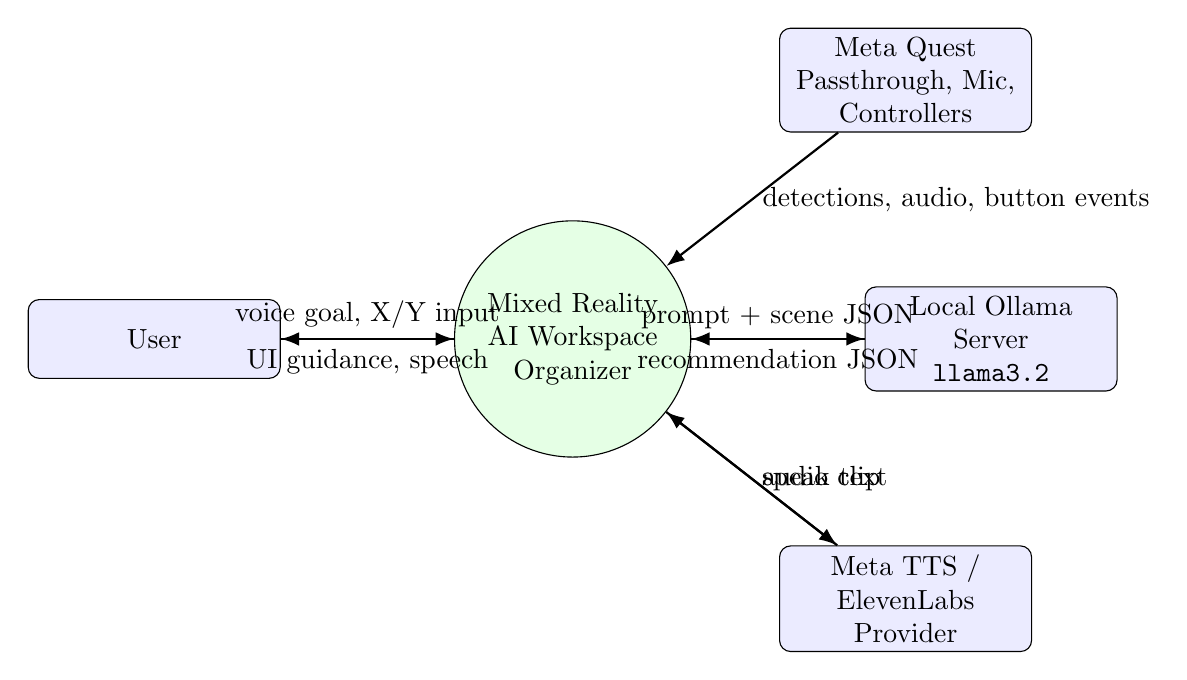
\begin{tikzpicture}[
    entity/.style={rectangle, draw, rounded corners, minimum width=3.2cm, minimum height=1cm, align=center, fill=blue!8},
    process/.style={circle, draw, minimum size=3cm, align=center, fill=green!10},
    data/.style={-Latex, thick},
    node distance=2.2cm
]
\node[entity] (user) {User};
\node[process, right=of user] (system) {Mixed Reality\\AI Workspace\\Organizer};
\node[entity, above right=of system] (sensors) {Meta Quest\\Passthrough, Mic,\\Controllers};
\node[entity, right=of system] (ollama) {Local Ollama\\Server\\\texttt{llama3.2}};
\node[entity, below right=of system] (tts) {Meta TTS /\\ElevenLabs\\Provider};

\draw[data] (user) -- node[above]{voice goal, X/Y input} (system);
\draw[data] (system) -- node[below]{UI guidance, speech} (user);
\draw[data] (sensors) -- node[right]{detections, audio, button events} (system);
\draw[data] (system) -- node[above]{prompt + scene JSON} (ollama);
\draw[data] (ollama) -- node[below]{recommendation JSON} (system);
\draw[data] (system) -- node[right]{speak text} (tts);
\draw[data] (tts) -- node[right]{audio clip} (system);
\end{tikzpicture}
\caption{DFD Level 0: Context diagram}
\end{figure}

\subsection{DFD Level 1}

DFD Level 1 expands the internal processing steps of the system.

\begin{figure}[h!]
\centering
\resizebox{\textwidth}{!}{
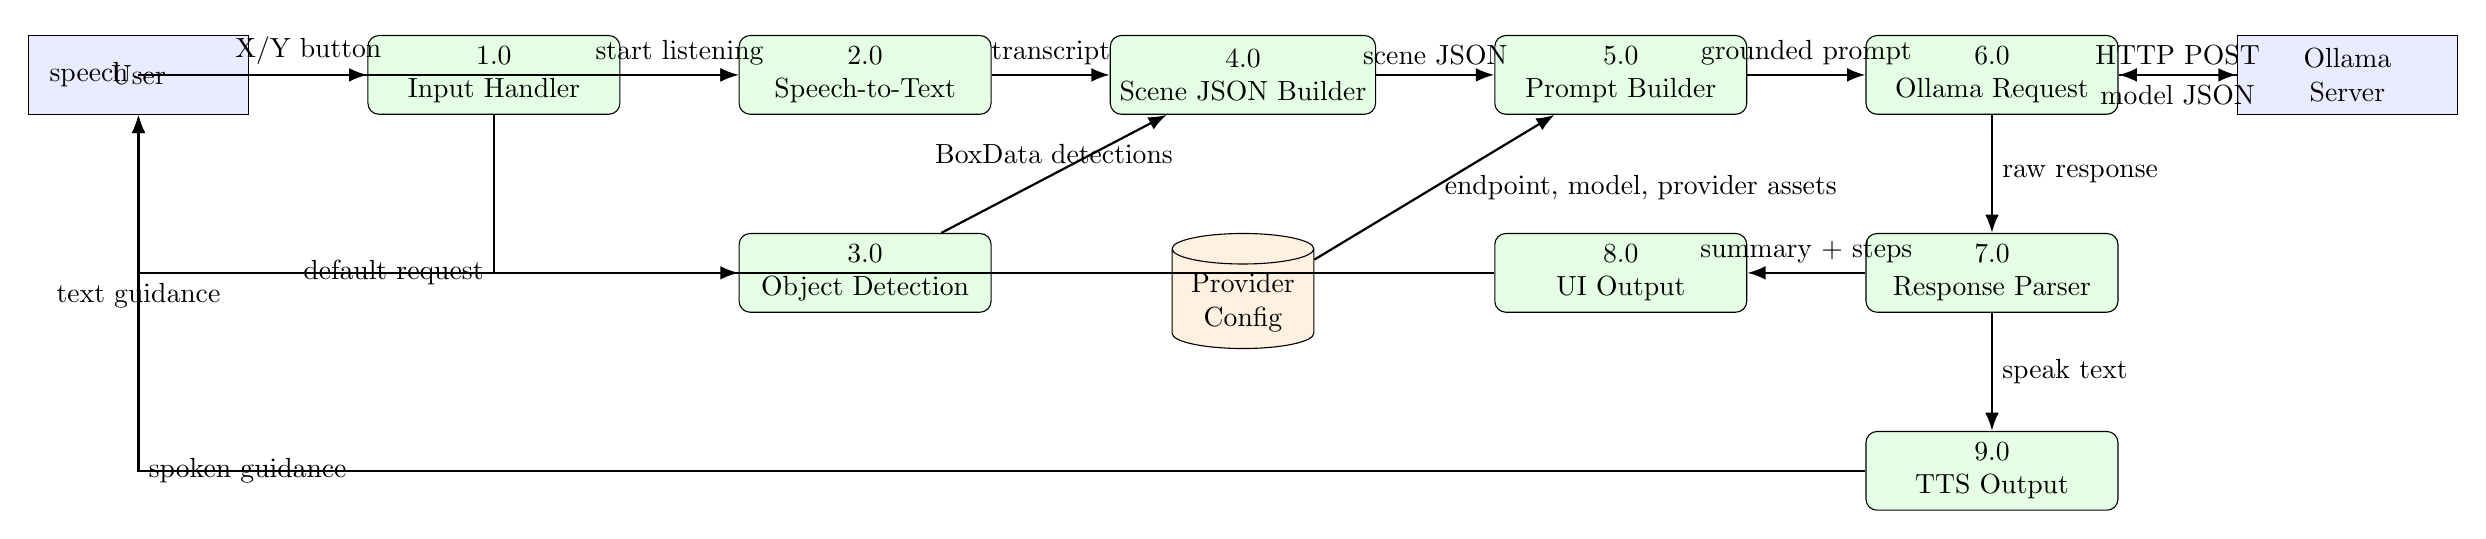
\begin{tikzpicture}[
    process/.style={rectangle, draw, rounded corners, minimum width=3.2cm, minimum height=1cm, align=center, fill=green!10},
    store/.style={cylinder, shape border rotate=90, draw, aspect=0.25, minimum height=1.1cm, minimum width=1.8cm, align=center, fill=orange!12},
    entity/.style={rectangle, draw, minimum width=2.8cm, minimum height=1cm, align=center, fill=blue!8},
    data/.style={-Latex, thick},
    node distance=1.5cm
]
\node[entity] (user) {User};
\node[process, right=of user] (input) {1.0\\Input Handler};
\node[process, right=of input] (stt) {2.0\\Speech-to-Text};
\node[process, below=of stt] (detect) {3.0\\Object Detection};
\node[process, right=of stt] (scene) {4.0\\Scene JSON Builder};
\node[store, below=of scene] (config) {Provider\\Config};
\node[process, right=of scene] (prompt) {5.0\\Prompt Builder};
\node[process, right=of prompt] (ollama) {6.0\\Ollama Request};
\node[entity, right=of ollama] (server) {Ollama\\Server};
\node[process, below=of ollama] (validate) {7.0\\Response Parser};
\node[process, left=of validate] (ui) {8.0\\UI Output};
\node[process, below=of validate] (voice) {9.0\\TTS Output};

\draw[data] (user) -- node[above]{X/Y button} (input);
\draw[data] (user) |- node[left]{speech} (stt);
\draw[data] (input) -- node[above]{start listening} (stt);
\draw[data] (input) |- node[left]{default request} (detect);
\draw[data] (stt) -- node[above]{transcript} (scene);
\draw[data] (detect) -- node[above]{BoxData detections} (scene);
\draw[data] (scene) -- node[above]{scene JSON} (prompt);
\draw[data] (config) -- node[right]{endpoint, model, provider assets} (prompt);
\draw[data] (prompt) -- node[above]{grounded prompt} (ollama);
\draw[data] (ollama) -- node[above]{HTTP POST} (server);
\draw[data] (server) -- node[below]{model JSON} (ollama);
\draw[data] (ollama) -- node[right]{raw response} (validate);
\draw[data] (validate) -- node[above]{summary + steps} (ui);
\draw[data] (validate) -- node[right]{speak text} (voice);
\draw[data] (ui) -| node[below]{text guidance} (user);
\draw[data] (voice) -| node[right]{spoken guidance} (user);
\end{tikzpicture}
}
\caption{DFD Level 1: Internal data flow}
\end{figure}

\section{Use Case Diagram}

\begin{figure}[h!]
\centering
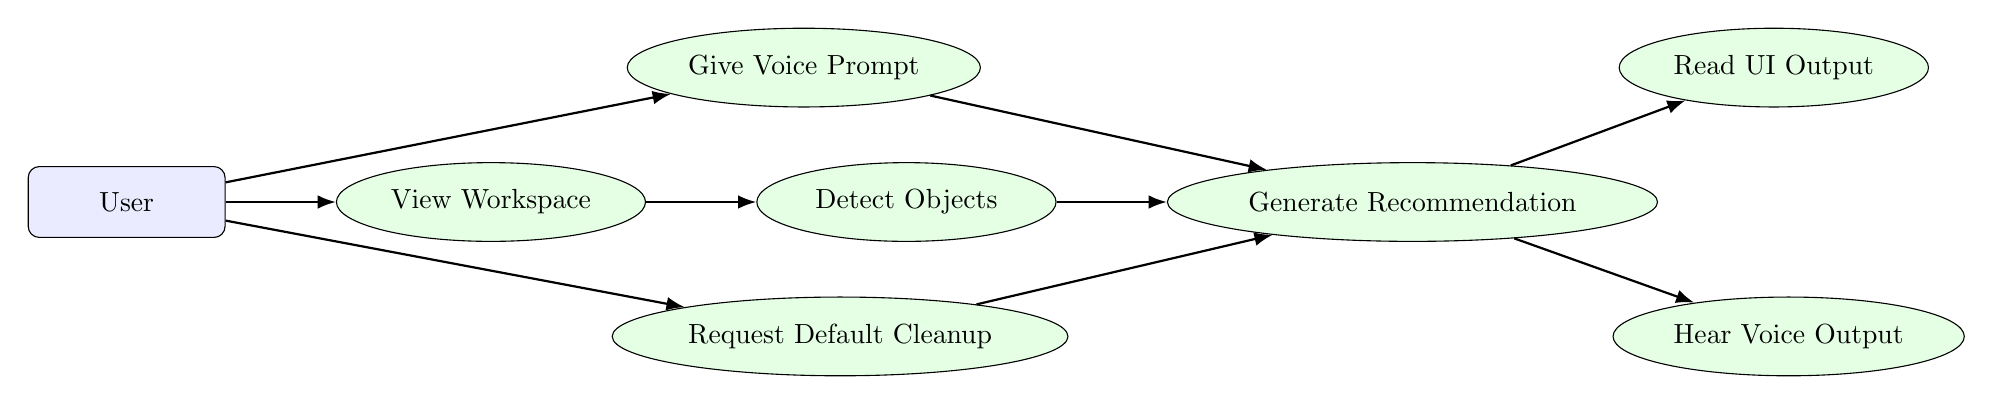
\begin{tikzpicture}[
    actor/.style={rectangle, draw, rounded corners, minimum width=2.5cm, minimum height=0.9cm, align=center, fill=blue!8},
    usecase/.style={ellipse, draw, minimum width=3.8cm, minimum height=1cm, align=center, fill=green!10},
    rel/.style={-Latex, thick},
    node distance=1.4cm
]
\node[actor] (user) {User};
\node[usecase, right=of user] (view) {View Workspace};
\node[usecase, above right=of view] (voice) {Give Voice Prompt};
\node[usecase, below right=of view] (default) {Request Default Cleanup};
\node[usecase, right=of view] (detect) {Detect Objects};
\node[usecase, right=of detect] (recommend) {Generate Recommendation};
\node[usecase, above right=of recommend] (ui) {Read UI Output};
\node[usecase, below right=of recommend] (tts) {Hear Voice Output};

\draw[rel] (user) -- (view);
\draw[rel] (user) -- (voice);
\draw[rel] (user) -- (default);
\draw[rel] (view) -- (detect);
\draw[rel] (voice) -- (recommend);
\draw[rel] (default) -- (recommend);
\draw[rel] (detect) -- (recommend);
\draw[rel] (recommend) -- (ui);
\draw[rel] (recommend) -- (tts);
\end{tikzpicture}
\caption{Use case diagram}
\end{figure}

\section{Sequence Diagram}

\begin{figure}[h!]
\centering
\resizebox{\textwidth}{!}{
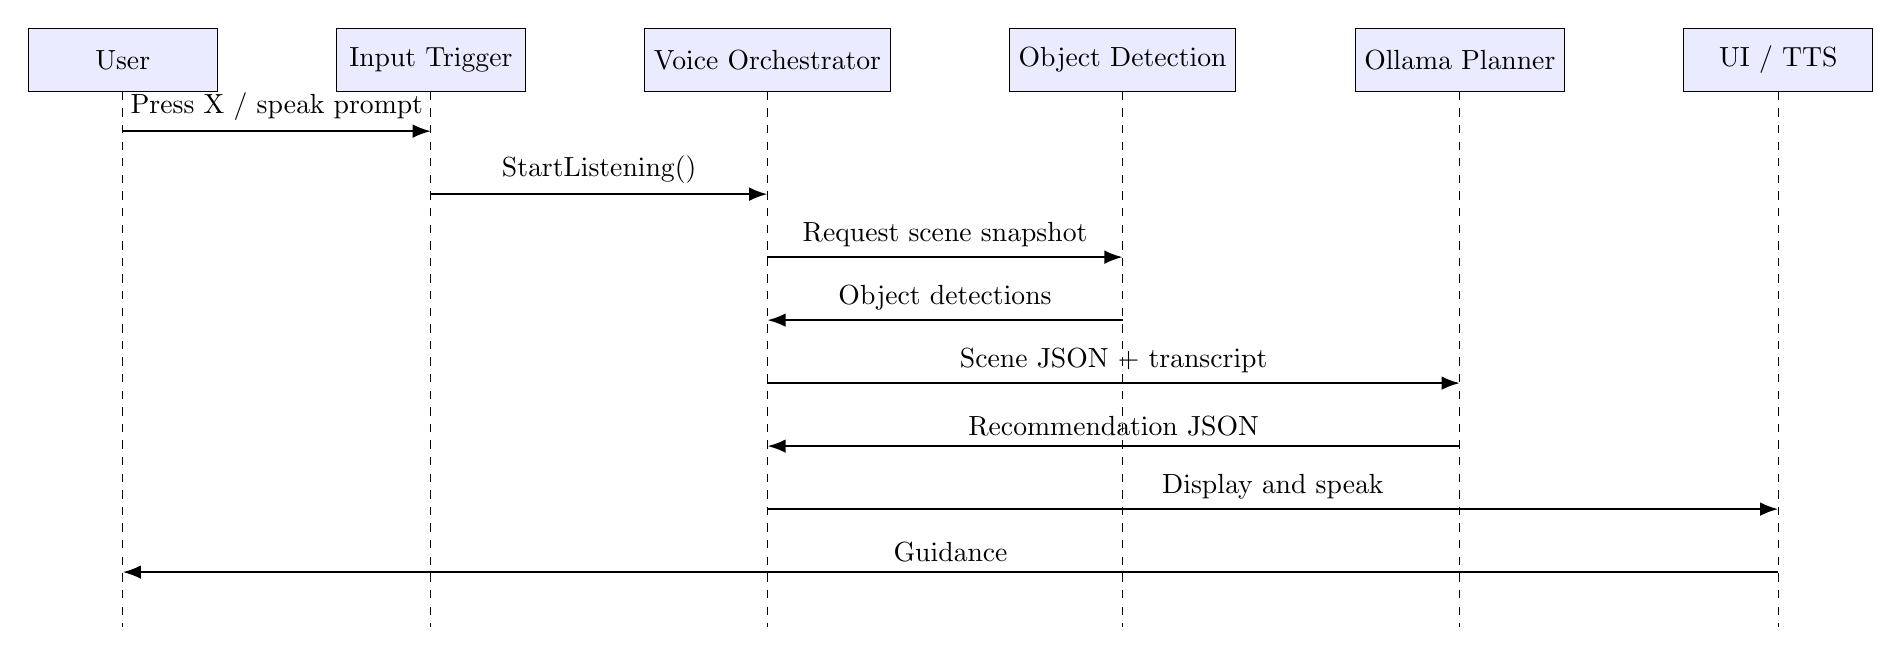
\begin{tikzpicture}[
    lifeline/.style={rectangle, draw, minimum width=2.4cm, minimum height=0.8cm, align=center, fill=blue!8},
    msg/.style={-Latex, thick},
    node distance=1.5cm
]
\node[lifeline] (user) {User};
\node[lifeline, right=of user] (input) {Input Trigger};
\node[lifeline, right=of input] (voice) {Voice Orchestrator};
\node[lifeline, right=of voice] (detect) {Object Detection};
\node[lifeline, right=of detect] (ollama) {Ollama Planner};
\node[lifeline, right=of ollama] (output) {UI / TTS};

\foreach \x in {user,input,voice,detect,ollama,output}
    \draw[dashed] (\x.south) -- ++(0,-6.8);

\draw[msg] ($(user.south)+(0,-0.5)$) -- node[above]{Press X / speak prompt} ($(input.south)+(0,-0.5)$);
\draw[msg] ($(input.south)+(0,-1.3)$) -- node[above]{StartListening()} ($(voice.south)+(0,-1.3)$);
\draw[msg] ($(voice.south)+(0,-2.1)$) -- node[above]{Request scene snapshot} ($(detect.south)+(0,-2.1)$);
\draw[msg] ($(detect.south)+(0,-2.9)$) -- node[above]{Object detections} ($(voice.south)+(0,-2.9)$);
\draw[msg] ($(voice.south)+(0,-3.7)$) -- node[above]{Scene JSON + transcript} ($(ollama.south)+(0,-3.7)$);
\draw[msg] ($(ollama.south)+(0,-4.5)$) -- node[above]{Recommendation JSON} ($(voice.south)+(0,-4.5)$);
\draw[msg] ($(voice.south)+(0,-5.3)$) -- node[above]{Display and speak} ($(output.south)+(0,-5.3)$);
\draw[msg] ($(output.south)+(0,-6.1)$) -- node[above]{Guidance} ($(user.south)+(0,-6.1)$);
\end{tikzpicture}
}
\caption{Sequence diagram for voice-guided recommendation}
\end{figure}

\section{Database and Data Design}

The current prototype does not require a persistent database. Runtime data is stored in memory as C\# objects and serialized JSON payloads. This design is suitable for a prototype because the main task is real-time recommendation rather than long-term record keeping.

\subsection{Main Runtime Data Structures}

\begin{longtable}{p{0.28\linewidth} p{0.62\linewidth}}
\toprule
\textbf{Data Structure} & \textbf{Fields}\\
\midrule
Detected Object & name, raw label, confidence, detection index, x, y, width, height, horizontal position, vertical position, size, zone.\\
Scene Data & surface, goal, list of detected objects, available zones, source.\\
Ollama Request & model name, prompt, stream flag, JSON format option.\\
Recommendation & summary, steps array, speak text.\\
\bottomrule
\end{longtable}

\subsection{Sample Scene JSON}

\begin{verbatim}
{
  "surface": "desk",
  "goal": "This place is cluttered and I want to clean it.",
  "objects": [
    {
      "name": "laptop",
      "zone": "center",
      "confidence": 0.91,
      "horizontalPosition": "center",
      "verticalPosition": "middle",
      "size": "large"
    },
    {
      "name": "keyboard",
      "zone": "bottom",
      "confidence": 0.86,
      "horizontalPosition": "center",
      "verticalPosition": "bottom",
      "size": "medium"
    }
  ],
  "source": "Meta ObjectDetectionAgent"
}
\end{verbatim}

\subsection{Expected Recommendation JSON}

\begin{verbatim}
{
  "summary": "Organize the main work area around the laptop.",
  "steps": [
    "Place the keyboard directly below the laptop in the center.",
    "Move the bottle to the right edge away from the laptop.",
    "Stack the books on the left side of the desk."
  ],
  "speak": "Keep the laptop centered and place the keyboard directly below it.
Move the bottle to the right edge, away from the electronics."
}
\end{verbatim}

\section{Prompt Engineering Design}

The system prompt is designed to reduce hallucination and force object-grounded output. The model is instructed to:

\begin{itemize}
    \item Use only object names present in \texttt{objects[].name}.
    \item Avoid inventing shelves, drawers, boxes, or furniture that was not detected.
    \item Use relative placement instructions when possible.
    \item Mention exact object relationships such as left of, right of, above, below, beside, group with, or separate from.
    \item Keep liquids away from electronics.
    \item Return valid JSON only.
\end{itemize}

This makes the LLM more reliable for a client environment because downstream UI and speech systems depend on a predictable response format.

\section{Agile Scrum Project Management}

\subsection{Scrum Roles}

\begin{longtable}{p{0.25\linewidth} p{0.65\linewidth}}
\toprule
\textbf{Role} & \textbf{Responsibility}\\
\midrule
Product Owner & Defines the user problem, prioritizes features, and validates whether recommendations are useful.\\
Scrum Master & Removes blockers such as device setup, network issues, package problems, and build failures.\\
Development Team & Implements Unity scripts, object detection integration, LLM prompt logic, UI, TTS, testing, and documentation.\\
Client / Stakeholder & Provides feedback on usability, desired recommendation style, and deployment requirements.\\
\bottomrule
\end{longtable}

\subsection{Product Backlog}

\begin{longtable}{p{0.12\linewidth} p{0.52\linewidth} p{0.18\linewidth} p{0.10\linewidth}}
\toprule
\textbf{ID} & \textbf{User Story} & \textbf{Priority} & \textbf{Status}\\
\midrule
US-01 & As a user, I want the headset to detect objects in my workspace so that the assistant understands my environment. & High & Done\\
US-02 & As a user, I want to press Y and get cleanup suggestions without speaking. & High & Done\\
US-03 & As a user, I want to press X and speak a custom organization goal. & High & Done\\
US-04 & As a user, I want recommendations to mention exact object placement. & High & Done\\
US-05 & As a user, I want the recommendation to appear in UI for debugging and accessibility. & High & Done\\
US-06 & As a user, I want the recommendation to be spoken aloud. & Medium & In Progress\\
US-07 & As a user, I want ghost previews showing where objects should be placed. & Medium & Prototype\\
US-08 & As a client, I want the model endpoint to be configurable for different deployments. & Medium & Done\\
US-09 & As a developer, I want clear logs for object detection, Ollama, STT, and TTS failures. & Medium & Done\\
US-10 & As a client, I want user profiles and saved workspace preferences. & Low & Future\\
\bottomrule
\end{longtable}

\subsection{Sprint Plan}

\begin{longtable}{p{0.18\linewidth} p{0.72\linewidth}}
\toprule
\textbf{Sprint} & \textbf{Planned Work}\\
\midrule
Sprint 1 & Unity project setup, Meta XR SDK setup, passthrough scene, object detection block integration.\\
Sprint 2 & Object detection event handling, scene JSON generation, Ollama endpoint configuration, initial UI output.\\
Sprint 3 & Speech-to-text pipeline, voice orchestrator, prompt builder, model response validation.\\
Sprint 4 & Text-to-speech integration, controller bindings, improved prompts, detailed recommendations.\\
Sprint 5 & Ghost preview prototype, testing on Quest, documentation, client scalability planning.\\
\bottomrule
\end{longtable}

\subsection{Definition of Done}

A feature is considered done when:

\begin{itemize}
    \item It compiles without C\# errors.
    \item It is wired into the Unity scene or documented as a script-level feature.
    \item It has clear logs for success and failure states.
    \item It does not break the existing object detection and Ollama flow.
    \item It can be tested either in the Unity editor, through debug transcript mode, or on the Quest headset.
\end{itemize}

\section{Coding Practices and Scalability}

\subsection{Modular Design}

The code is separated into focused components. For example, \texttt{SpeechInputManager} only handles speech input, \texttt{SceneContextBuilder} only builds scene data and prompts, and \texttt{SpeechOutputManager} only handles voice output. This improves maintainability because a client can replace one provider without rewriting the entire workflow.

\subsection{Event-Driven Communication}

Unity events and C\# events are used to connect components. This reduces tight coupling between scripts and allows UI, TTS, and debugging systems to subscribe to recommendation events independently.

\subsection{Configuration Through Assets}

Provider assets store model and API configuration, such as Ollama endpoint, speech provider, TTS provider, and object detection model. This makes deployment easier for different client environments.

\subsection{Structured API Contracts}

The system expects a strict JSON schema from Ollama. This makes the AI response usable by UI and TTS components and prevents free-form text from breaking downstream logic.

\subsection{Error Handling}

The system reports errors for missing components, empty speech input, missing model name, unreachable Ollama endpoint, request timeouts, and invalid model responses. These logs are important for client support and testing.

\subsection{Scalability for Client Deployment}

The project can be scaled by:

\begin{itemize}
    \item Replacing local Ollama with a dedicated backend service.
    \item Adding authentication and user accounts.
    \item Saving user preferences and room profiles.
    \item Supporting multiple language models through an interface.
    \item Adding analytics for recommendation usefulness.
    \item Expanding ghost previews into interactive placement confirmation.
    \item Adding localization for multiple spoken languages.
\end{itemize}

\section{Testing Strategy}

\subsection{Unit-Level Testing}

The following components can be tested individually:

\begin{itemize}
    \item JSON generation from sample detections.
    \item Prompt construction using mock scene data.
    \item Ollama response parsing and validation.
    \item Input trigger state transitions.
    \item UI formatting for recommendations.
\end{itemize}

\subsection{Integration Testing}

Integration tests should verify:

\begin{itemize}
    \item Object detection output reaches the scene builder.
    \item Scene JSON reaches Ollama.
    \item Ollama returns valid JSON.
    \item UI displays the response.
    \item TTS receives the \texttt{speak} field.
    \item X and Y controller bindings trigger the correct workflows.
\end{itemize}

\subsection{System Testing}

System testing should be performed on the Quest headset in a real workspace. Test cases should include:

\begin{longtable}{p{0.14\linewidth} p{0.45\linewidth} p{0.31\linewidth}}
\toprule
\textbf{Test ID} & \textbf{Scenario} & \textbf{Expected Result}\\
\midrule
TC-01 & Press Y while looking at a workspace. & The system detects objects and shows default cleanup suggestions.\\
TC-02 & Press X and say a custom prompt. & The system uses the transcript and detected scene to generate suggestions.\\
TC-03 & Ollama server is stopped. & The system shows a clear connection error.\\
TC-04 & No objects are detected. & The system says no detected objects are available yet.\\
TC-05 & TTS provider fails. & The UI still displays the recommendation and logs the TTS error.\\
TC-06 & User presses X while listening. & The system stops recording and allows STT to process.\\
\bottomrule
\end{longtable}

\section{Risk Management}

\begin{longtable}{p{0.24\linewidth} p{0.36\linewidth} p{0.30\linewidth}}
\toprule
\textbf{Risk} & \textbf{Impact} & \textbf{Mitigation}\\
\midrule
Object detection misses objects & Recommendations may be incomplete. & Prompt model to only use detected objects and ask user to look at workspace again.\\
Ollama network timeout & No recommendation generated. & Increase request timeout and show clear error.\\
Quest cannot reach PC server & Ollama calls fail in headset build. & Use PC LAN IP instead of localhost and enable Android internet permissions.\\
TTS API permission issue & Voice output may not play. & Keep UI output as fallback and verify TTS provider permissions.\\
Model hallucination & Incorrect object placement advice. & Use strict prompt constraints and response validation.\\
Overlapping requests & Confusing UI and audio states. & Use request-in-flight guards in orchestrator.\\
\bottomrule
\end{longtable}

\section{Security and Privacy Considerations}

The project handles microphone input and physical scene information. For client deployment, privacy must be considered carefully.

\begin{itemize}
    \item API keys should not be hardcoded in public source code.
    \item Voice transcripts should not be stored unless the user consents.
    \item If a cloud model is used later, the client should be informed that scene descriptions may leave the device/network.
    \item Local Ollama deployment improves privacy because prompts can remain on the local network.
    \item Android permissions should be limited to only what the application needs.
\end{itemize}

\section{Limitations}

\begin{itemize}
    \item The quality of recommendations depends on object detection accuracy.
    \item The object detector may not understand every object category.
    \item The current prototype does not save long-term workspace state.
    \item Ghost placement is scaffolded but not yet a fully completed user workflow.
    \item TTS depends on correct provider permissions and available API credits.
    \item Local Ollama requires the Quest and PC to be on a reachable network.
\end{itemize}

\section{Future Enhancements}

\begin{itemize}
    \item Add persistent user profiles and workspace preferences.
    \item Add before-and-after workspace scoring.
    \item Add interactive ghost placement previews with confirmation.
    \item Add hand tracking for selecting objects.
    \item Add multiple model provider support.
    \item Add cloud deployment option for enterprise clients.
    \item Add multilingual speech input and output.
    \item Add accessibility modes with larger UI, slower speech, and repeated instructions.
\end{itemize}

\section{Placeholder for Project Images}

The following figure placeholders can be replaced with screenshots later.

\begin{figure}[h!]
\centering
\fbox{\parbox[c][6cm][c]{0.8\linewidth}{\centering Add screenshot of Meta Quest passthrough object detection here.}}
\caption{Passthrough and object detection view}
\end{figure}

\begin{figure}[h!]
\centering
\fbox{\parbox[c][6cm][c]{0.8\linewidth}{\centering Add screenshot of UI recommendation output here.}}
\caption{Generated recommendation displayed in UI}
\end{figure}

\begin{figure}[h!]
\centering
\fbox{\parbox[c][6cm][c]{0.8\linewidth}{\centering Add screenshot of Unity scene hierarchy or manager components here.}}
\caption{Unity scene setup}
\end{figure}

\section{Conclusion}

The Mixed Reality AI Workspace Organizer demonstrates how software engineering principles can be applied to a modern AI and XR application. The project integrates perception, language understanding, voice interaction, and mixed reality output in a modular Unity architecture. It provides practical object-specific workspace recommendations and is designed so that future client requirements can be added without rewriting the whole system.

The project is also suitable for a software engineering course because it includes requirements analysis, modular architecture, DFD modeling, agile Scrum planning, testing strategy, risk management, and scalability planning. These practices make the prototype more maintainable and closer to a real client-ready software product.

\end{document}
